% !TeX root = ../main.tex

%\section{Simulation Study}

We base the simulated study on acceleration data of a killer whale dive sequence. The parameters used in this simulation study are loosely based on those learned from the case study in section \ref{sec:case_study}.

\subsection{Data Simulation}

500 separate sequences of 100 killer whale dives were simulated according to an HMM, where the hidden Markov chain $X$ was set as a collection of dive types and the observations $Y$ were the corresponding dive durations (in seconds). Each dive could be one of $N=2$ dive types, and the duration of dive $t$, $Y_t$, followed a gamma distribution whose parameters $\theta^{(i)}$ depended upon the dive type $X_t = i$. We parameterize the gamma distribution by its mean and variance:

$$\Gamma = \begin{pmatrix} 0.5 & 0.5 \\ 0.5 & 0.5 \end{pmatrix}, \qquad \delta =  \begin{pmatrix} 0.5 & 0.5 \end{pmatrix}$$
$$Y_t|X_t \sim \rm{Gamma} $$
\begin{align*}
	&\bbE(Y_t|X_t = 1) = 15 s &\bbE(Y_t|X_t = 2) = 60 s \\
	%
	&\bbV(Y_t|X_t = 1) = 25 s^2 &\bbV(Y_t|X_t = 2) = 100 s^2
\end{align*}

Once the dive durations were calculated for all 100 dives, dive $t$ was broken into a sequence of $T^*_t = \lfloor Y_t/2 \rfloor$ two-second segments (the end of the dive sequence was discarded) which made up a second fine-scale hidden Markov model. Each 2-second segment of the dive was assigned one of $N^*=2$ behaviours (active swimming or passive gliding) according to a fine-scale Markov chain $X^*_t \equiv \left(X^*_{t,1}, \ldots, X^*_{t,T^*_t} \right)$, and the probability transition matrices for these fine-scale Markov chains were set as follows:
%
$$\Gamma^{*(1)} = \begin{pmatrix} 0.5 & 0.5 \\ 0.9 & 0.1 \end{pmatrix} \qquad \Gamma^{*(2)} = \begin{pmatrix} 0.8 & 0.2 \\ 0.3 & 0.7 \end{pmatrix}$$
%
where $\Gamma^{*(1)}$ was used for dives where $X_t = 1$ and $\Gamma^{*(2)}$ was used for dives where $X_t = 2$. 

Each two-second sub-dive window had 100 associated acceleration readings, $Y^*_{t,t^*} \equiv \left(Y^*_{t,t^*,1}, \ldots, Y^*_{t,t^*,100}\right)$. To accurately recreate active swimming vs passive gliding on the fine-scale Markov chain, the DFT of each 2-second segment $\hat Y^*_{t,t^*}$ was simulated such that $Z^{*(1)}_{t,t^*}$ and $Z^{*(2)}_{t,t^*}$ (see eqn \ref{eqn:z}) would have the following distributions: 

\begin{align*}
    \left(Z^{*(1)}_{t,t^*} | Z^{*(1)}_{t,t^*-1}, X^*_{t,t^*} = 1 \right) &\sim \mathcal{N} \left(\phi^{*(1)}Z^{*(1)}_{t,t^*-1} + (1-\phi^{*(1)})\mu^{*(1)}, (\sigma^{*(1)})^2 \right) \\
    %
    \left(Z^{*(1)}_{t,t^*} | Z^{*(1)}_{t,t^*-1}, X^*_{t,t^*} = 2 \right) &\sim \mathcal{N} \left(\phi^{*(2)}Z^{*(1)}_{t,t^*-1} + (1-\phi^{*(2)})\mu^{*(2)}, (\sigma^{*(2)})^2 \right) \\
    %
    \mu^{*(1)} = 0.0,\enspace \sigma^{*(1)} &= 0.05,\enspace \phi^{*(1)} = 0.99 \\
    %
    \mu^{*(2)} = 0.0,\enspace \sigma^{*(2)} &= 0.1,\enspace \phi^{*(2)} = 0.95 \\\\
    %
    \left(Z^{*(2)}_{t,t^*} | X^*_{t,t^*} = 1\right) &\sim {\rm{Gamma}}\left(\alpha^{*(1)}, \beta^{*(1)} \right) \\
    %
    \left(Z^{*(2)}_{t,t^*} | X^*_{t,t^*} = 2\right) &\sim {\rm{Gamma}}\left(\alpha^{*(2)}, \beta^{*(2)} \right) \\
    %
    \alpha^{*(1)} = 10.10, \enspace & \enspace \beta^{*(1)} = 1.00 \\
    %
    \alpha^{*(2)} = 305.94, \enspace & \enspace \beta^{*(2)} = 1.00
\end{align*}
%
In short, sub-dive behavior 1 corresponds to passive gliding while sub-dive behaviour 2 corresponds to active swimming at a frequency of 1 hertz. In addition, sub-dive behaviors 1 and 2 are the same for both dive types. See the appendix for more details regarding procedure for simulating $\hat Y^*$ and $Y^*$ in addition to $Z^*$. (fig. \ref{fig:sim_data}) shows the first 5 dives of one simulated data set.

\begin{figure}[ht]
	\centering
	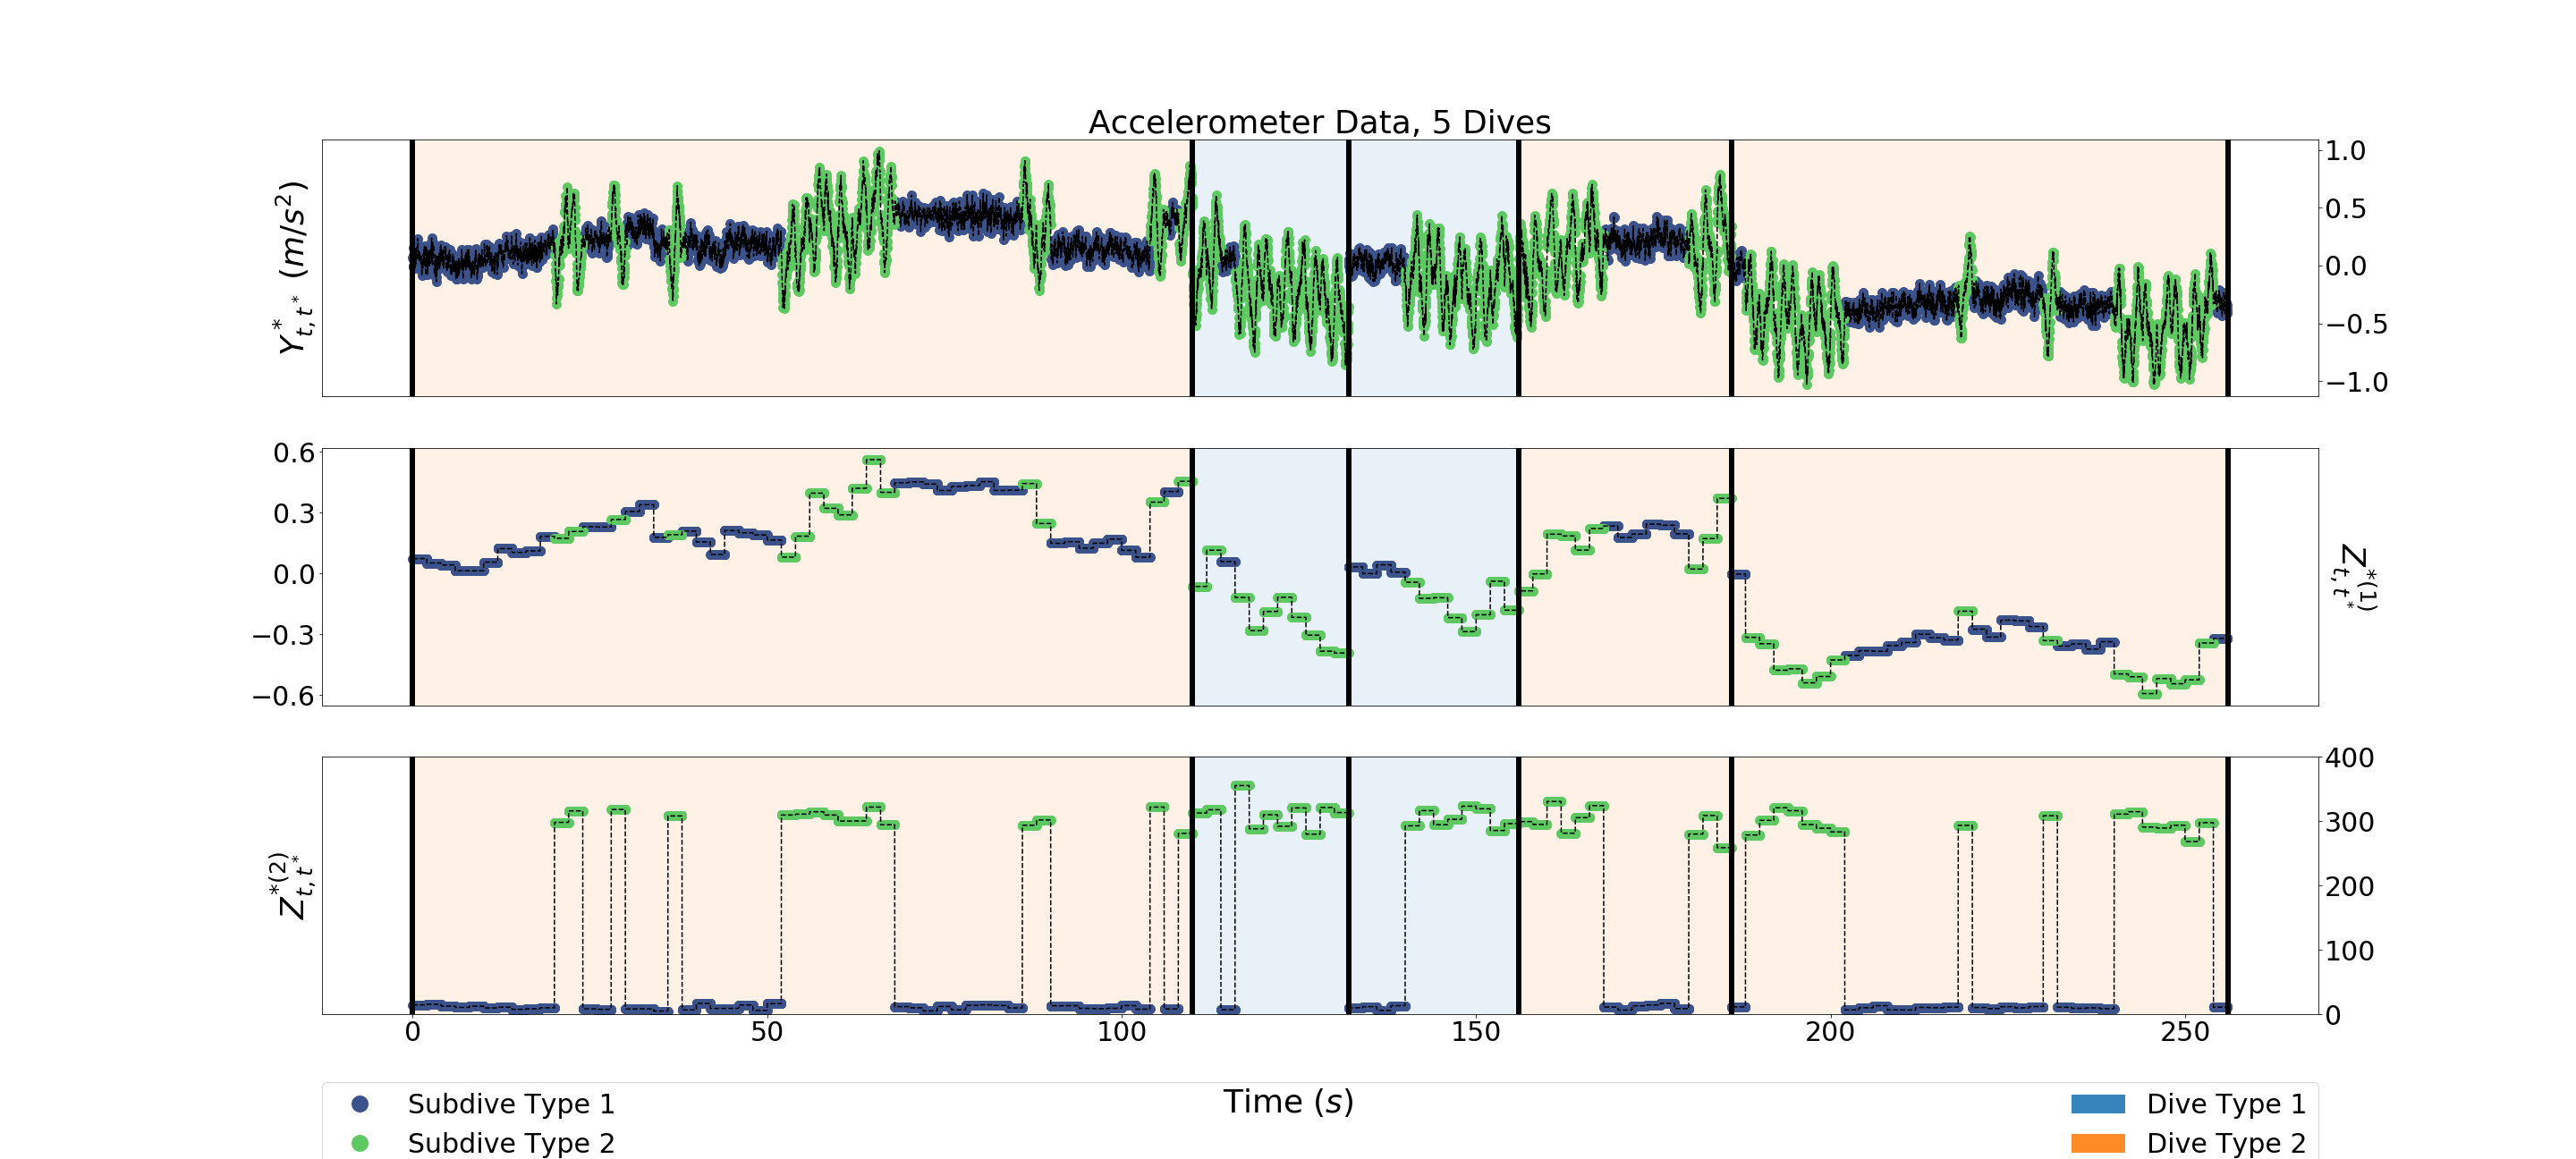
\includegraphics[width=5in]{../Plots/sim_data.png}
	\caption{Simulated acceleration data for one dive. The color of the line corresponds to the true fine-scale state of the sub-dive process, while the color of the background corresponds to the true dive type of the simulated whale, where blue corresponds to dive type 1 and orange corresponds to dive type 2.}
	\label{fig:sim_data}
\end{figure}

\subsection{Model Formulation}
\label{subsec:model_structure}

The building blocks from the previous section were used to build a well-specified model for this simulated data. Specifically, we used a hierarchical HMM where the sequence of dive durations $Y$ was modeled using a simple HMM, and the fine-scale process $Z^*$ was modeled using a HMM-DFT with explicit auto-correlation in $Z^{*(1)}$. Naturally, we refer to this model as the \textit{CarHHMM-DFT}, and (Fig. \ref{fig:CarHHMM}) shows the corresponding graphical model.
%
\begin{figure}[ht]
	\centering
	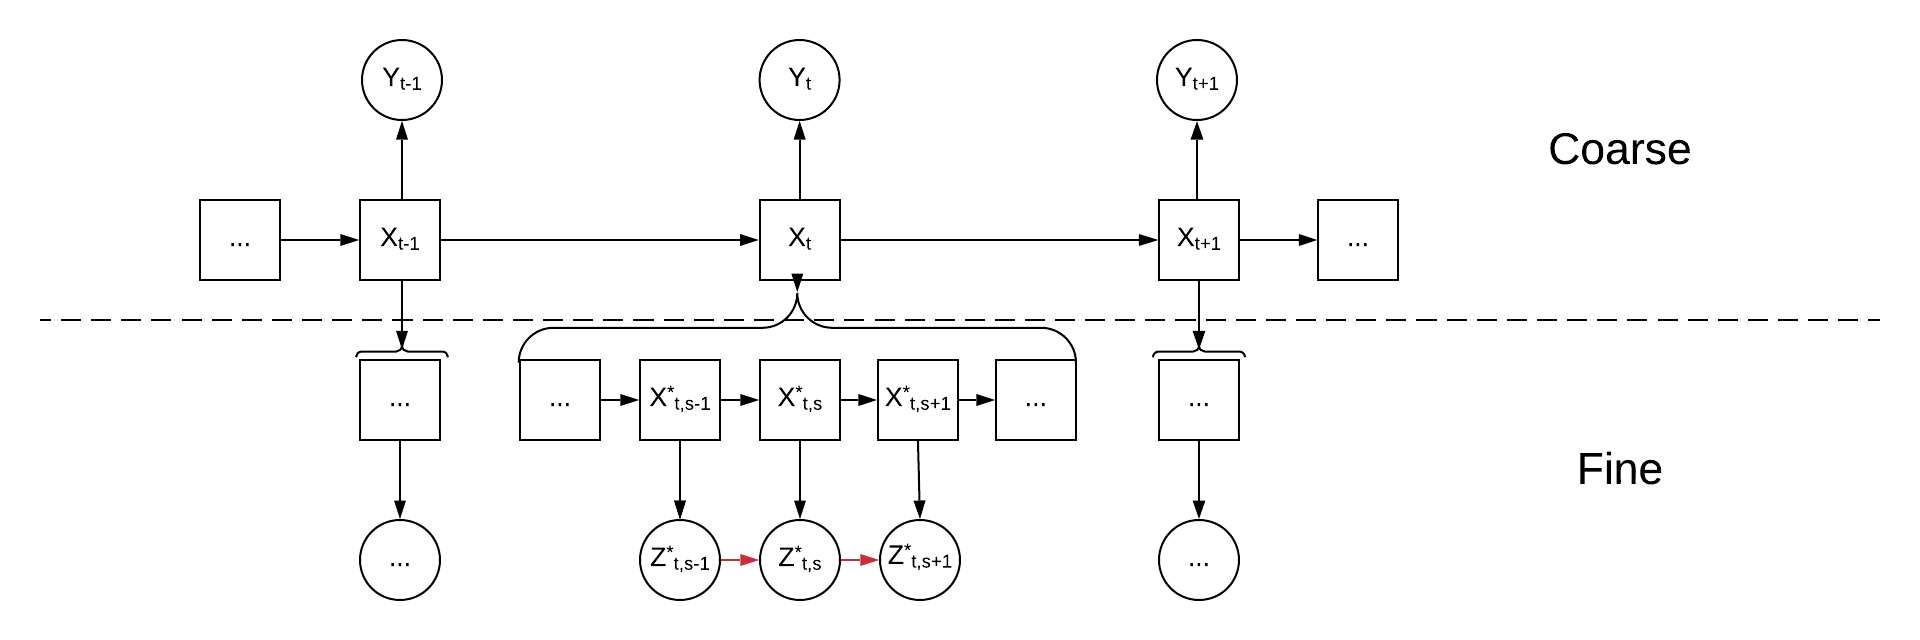
\includegraphics[width=5in]{../Plots/CarHHMM.png}
	\caption{Graphical representation of this model.}
	\label{fig:CarHHMM}
\end{figure}
%

\subsection{Parameters}

On the coarse scale, the dive types follow a Markov chain with $N=2$ possible states and unknown probability transition matrix $\Gamma$. Given the dive type, the duration of a dive follows a gamma distribution which depends upon the dive type and unknown parameters $\Theta = \{\{\mu^{(1)},\sigma^{(1)}\},\{\mu^{(2)},\sigma^{(2)}\}\}$.

On the fine scale, the sub-dive behavior of each two-second window comprises a Markov chain with $N^*=2$ possible states and unknown probability transition matrices $\Gamma^{*(1)}$ and $\Gamma^{*(2)}$, depending upon the dive type. Each two-second window is summarized by the observations $Z^{*(1)}_{t,t^*}$ and $Z^{*(2)}_{t,t^*}$. $Z^{*(1)}_{t,t^*}$ follows a normal distribution whose parameters depend upon the sub-dive behavior $X^*_{t,t^*}$ and $Z^{*(1)}_{t,t^*-1}$. In particular:

$$\mathbb{E}(Z^{*(1)}_{t,t^*}|Z^{*(1)}_{t,t^*-1} = z,X^*_{t,t^*} = i^*) = \phi_1^{*(i^*)}z + (1-\phi_1^{*(i^*)}) \mu_1^{*(i^*)}$$
$$\mathbb{V}(Z^{*(1)}_{t,t^*}|Z^{*(1)}_{t,t^*-1} = z,X^*_{t,t^*} = i^*) = \left(\sigma_1^{*(i^*)}\right)^2$$
%
$Z^{*(2)}_{t,t^*}$ follows a gamma distribution whose parameters depend upon only $X^*-{t,t^*}$:
%
$$\mathbb{E}(Z^{*(2)}_{t,t^*}|Z^{*(1)}_{t,t^*-1} = z,X^*_{t,t^*} = i^*) = \mu_2^{*(i^*)}$$
$$\mathbb{V}(Z^{*(2)}_{t,t^*}|Z^{*(1)}_{t,t^*-1} = z,X^*_{t,t^*} = i^*) = (\sigma_2^{*(i^*)})^2$$
%
None of the fine-scale emission distributions depend upon dive type. In total the parameters to learn are:

$$\Gamma, \qquad \Gamma^{*} = \{\Gamma^{*(1)},\Gamma^{*(2)}\} \qquad \text{(probability transition matrices)}$$
$$\Theta = \{\{\mu^{(1)},\sigma^{(1)}\},\{\mu^{(2)},\sigma^{(2)}\}\} \qquad \text{(coarse-scale emission parameters)}$$
$$\Theta^* = \{\Theta^{*(1)},\Theta^{*(2)}\}  \qquad \text{(fine-scale emission parameters)}$$
$$\Theta^{*(i^*)} =  \{\{\mu_1^{*(i^*)},\sigma_1^{*(i^*)},\phi_1^{*(i^*)}\},\{\mu_2^{*(i^*)},\sigma_2^{*(i^*)}\}\} \qquad \text{(}Z^{*(1)} \text{ and } Z^{*(2)} \text{ parameters)}$$

The likelihood of this model is still easy to calculate using the forward algorithm, and can be maximized with respect to the parameters above. See the appendix for details of likelihood evaluation.

Including the one described above, four different models were fit to the simulated data sets:

\begin{enumerate}
    \item A CarHHMM-DFT as described above (\textbf{CarHHMM-DFT}).
    \item An HHMM-DFT, which is similar to the model above, but with no modeled auto-correlation, i.e. $\phi_1^{*(i^*)} = 0$ for $i^* = 1,2$ (\textbf{HHMM-DFT}).
    \item A CarHHMM, which is similar to the model above, but which does not have access to $Z^{*(2)}$, i.e $\Theta^{*(i^*)} = \{\mu_1^{(i^*)},\sigma_1^{(i^*)},\phi_1^{(i^*)}\}$, $i^* = 1,2$ (\textbf{CarHHMM}).
    \item A CarHMM-DFT similar to the CarHHMM-DFT, but with $N=1$ instead of $N=2$, i.e. $\Gamma^* = \{\Gamma^{*(1)}\}$ and $\Theta^* = \{\Theta^{*(1)}\}$ (\textbf{CarHMM-DFT}). This is 
\end{enumerate}
%
Each of the last three models leaves out one important aspect of the full model (CarHHMM-DFT). The CarHMM-DFT lacks a hierarchical structure, the HHMM-DFT is missing auto-correlation within the fine-scale observations, and the CarHHMM does not have access to the Fourier transform sums $Z^{*(2)}$ as observations. All models were run on the Cedar Compute Canada cluster with 1 GPU and 4 GB of dedicated memory per model.

\subsection{Simulation Results}

%%% Accuracy %%%
Every model was able to decode the fine-scale hidden states of the process almost perfectly except for the \textit{CarHHMM}, which did not have access to the Fourier modes $Z^{*(2)}$. This is intuitively clear because the fine-scale states are much more distinct in their Fourier modes than in their average acceleration. For the coarse-scale hidden state, the CarHMM lacked a hierarchical structure and could not make any predictions at all. The other three models all achieved an accuracy of approximately 90\%, with the CarHHMM slightly more likely to categorize a dive as dive type 2 than the other models. (Fig. \ref{fig:acc}) shows the decoded state probabilities of both the fine and coarse hidden states for the first 5 dives of one simulated data set. (Tbl. \ref{table:accuracy}) also lists more details regarding the accuracy and training times of each model for each true dive and sub-dive state.

\begin{figure}[ht]
    \centering
    \begin{subfigure}[t]{1.0\textwidth}
        \centering
        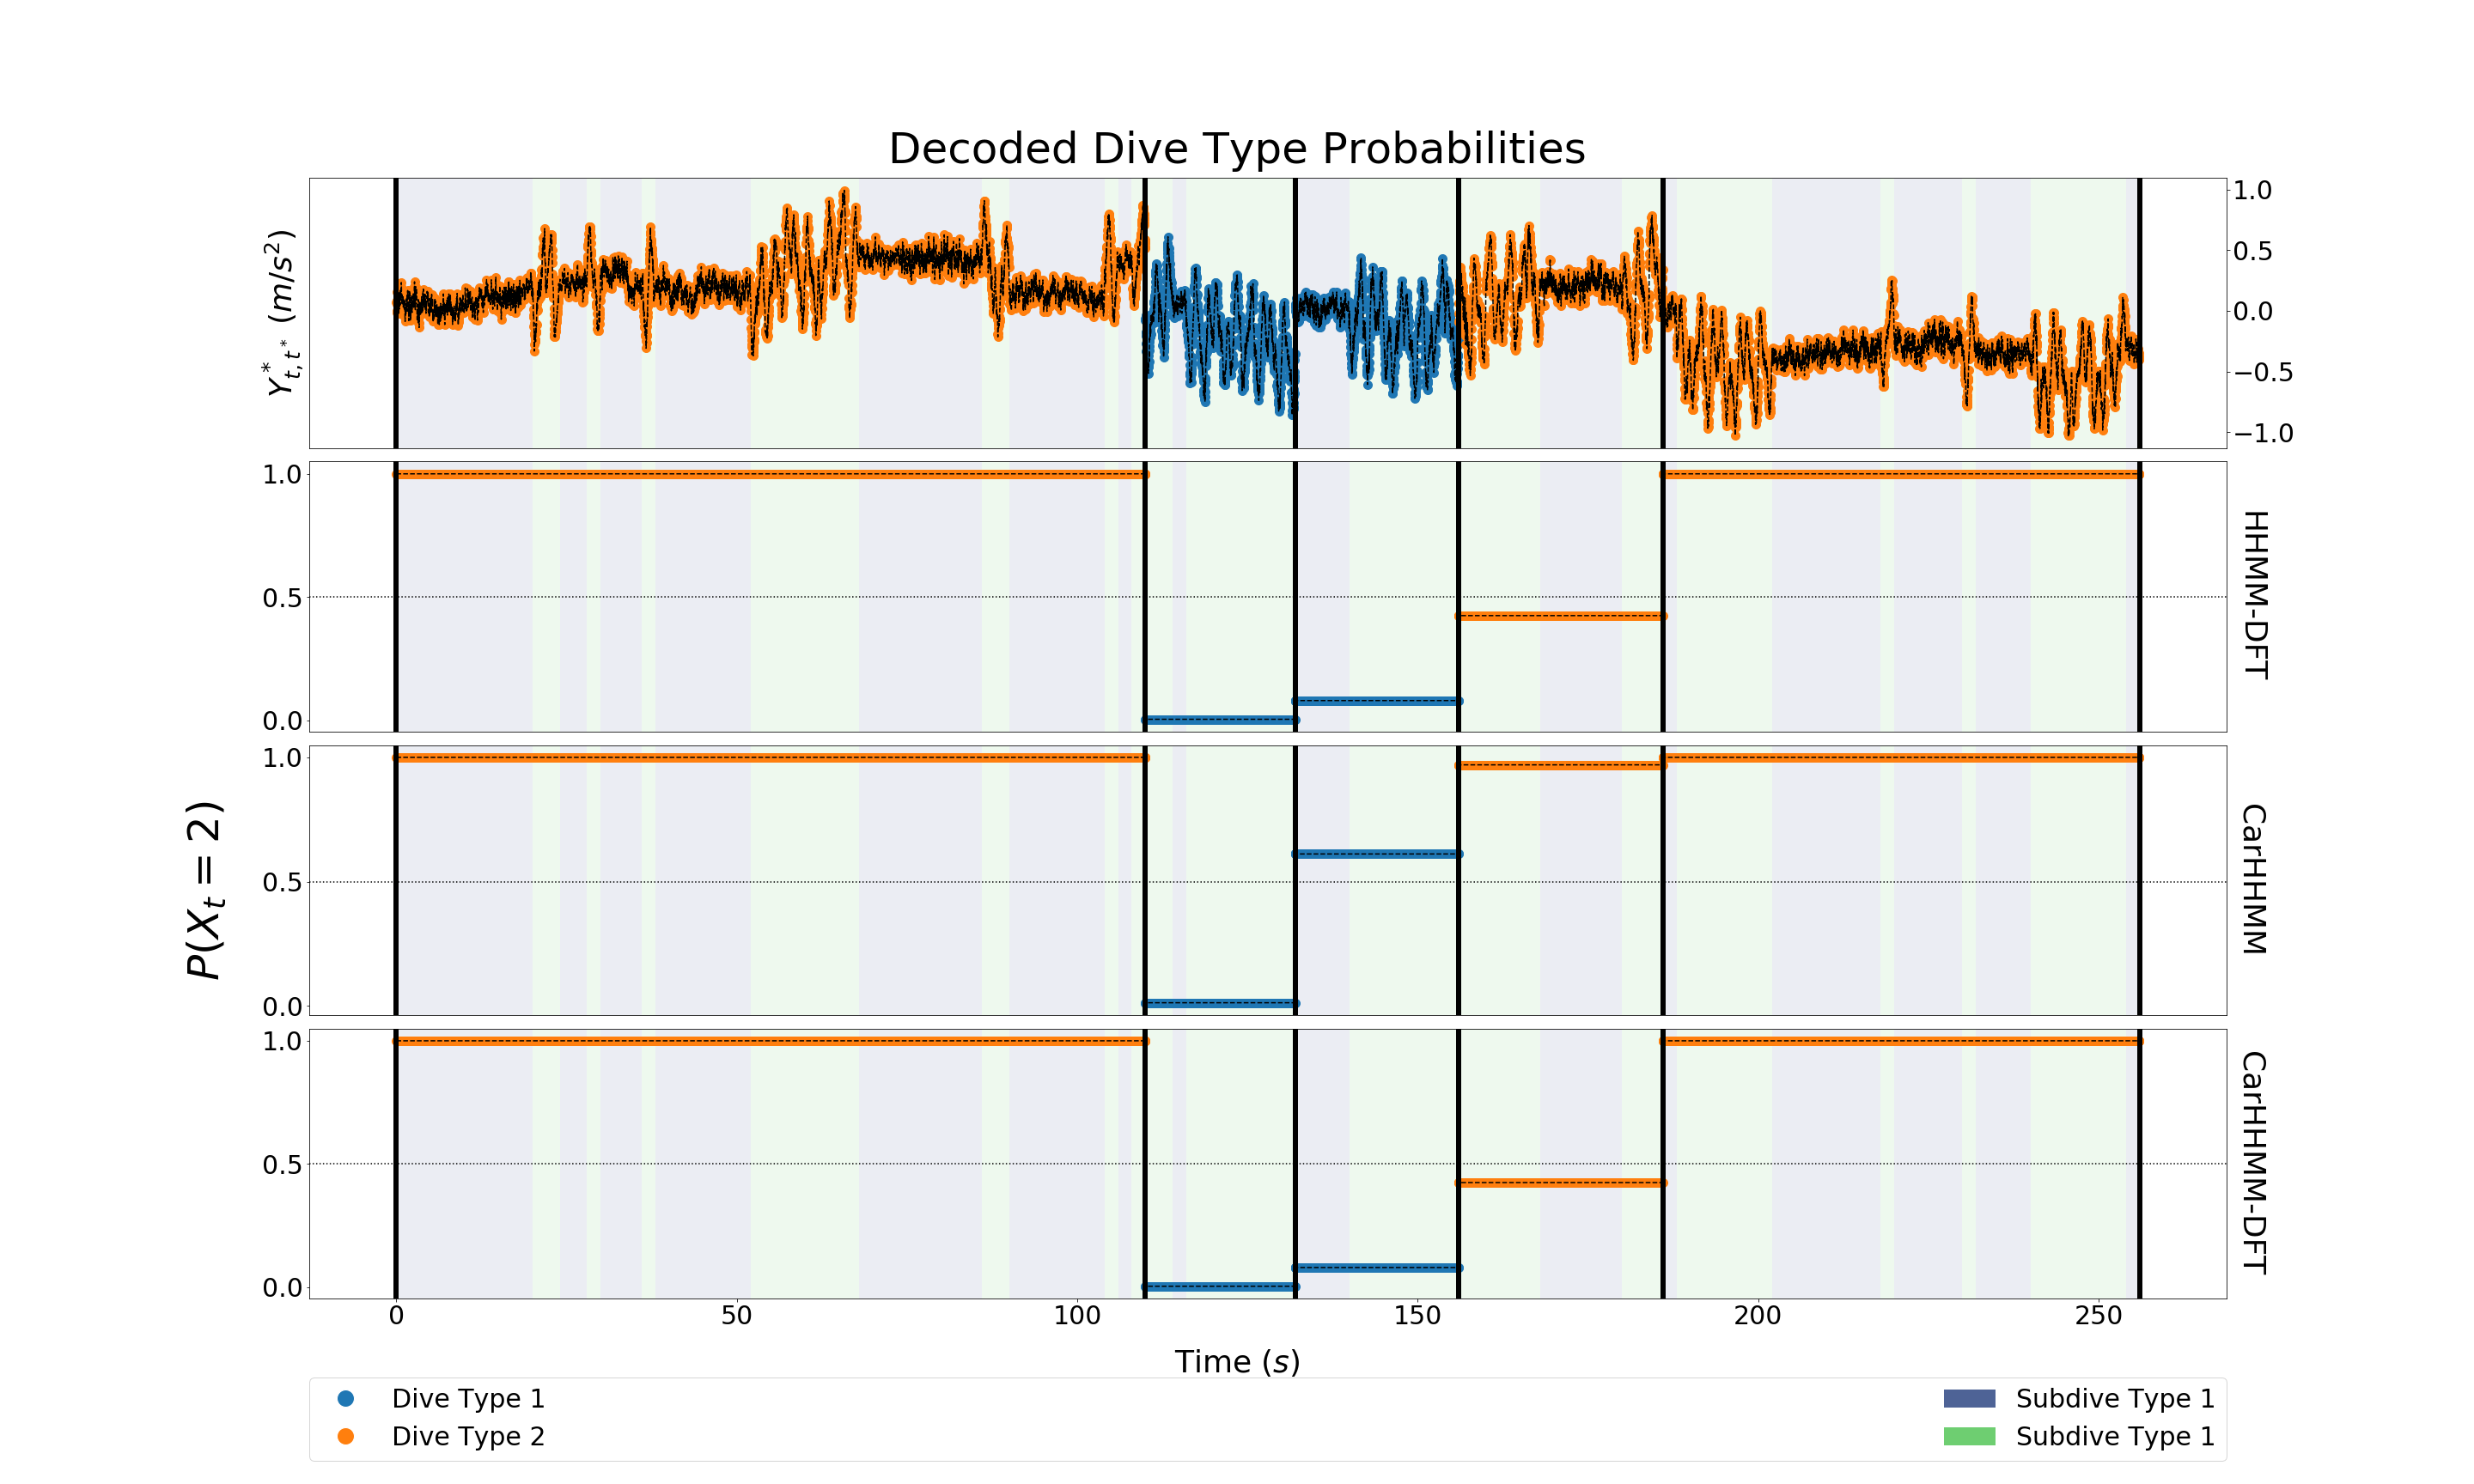
\includegraphics[width=5in]{Plots/Posterior_Coarse_States.png}
        \caption{Coarse-scale hidden process}
    \end{subfigure}
    \newline
    \begin{subfigure}[t]{1.0\textwidth}
        \centering
        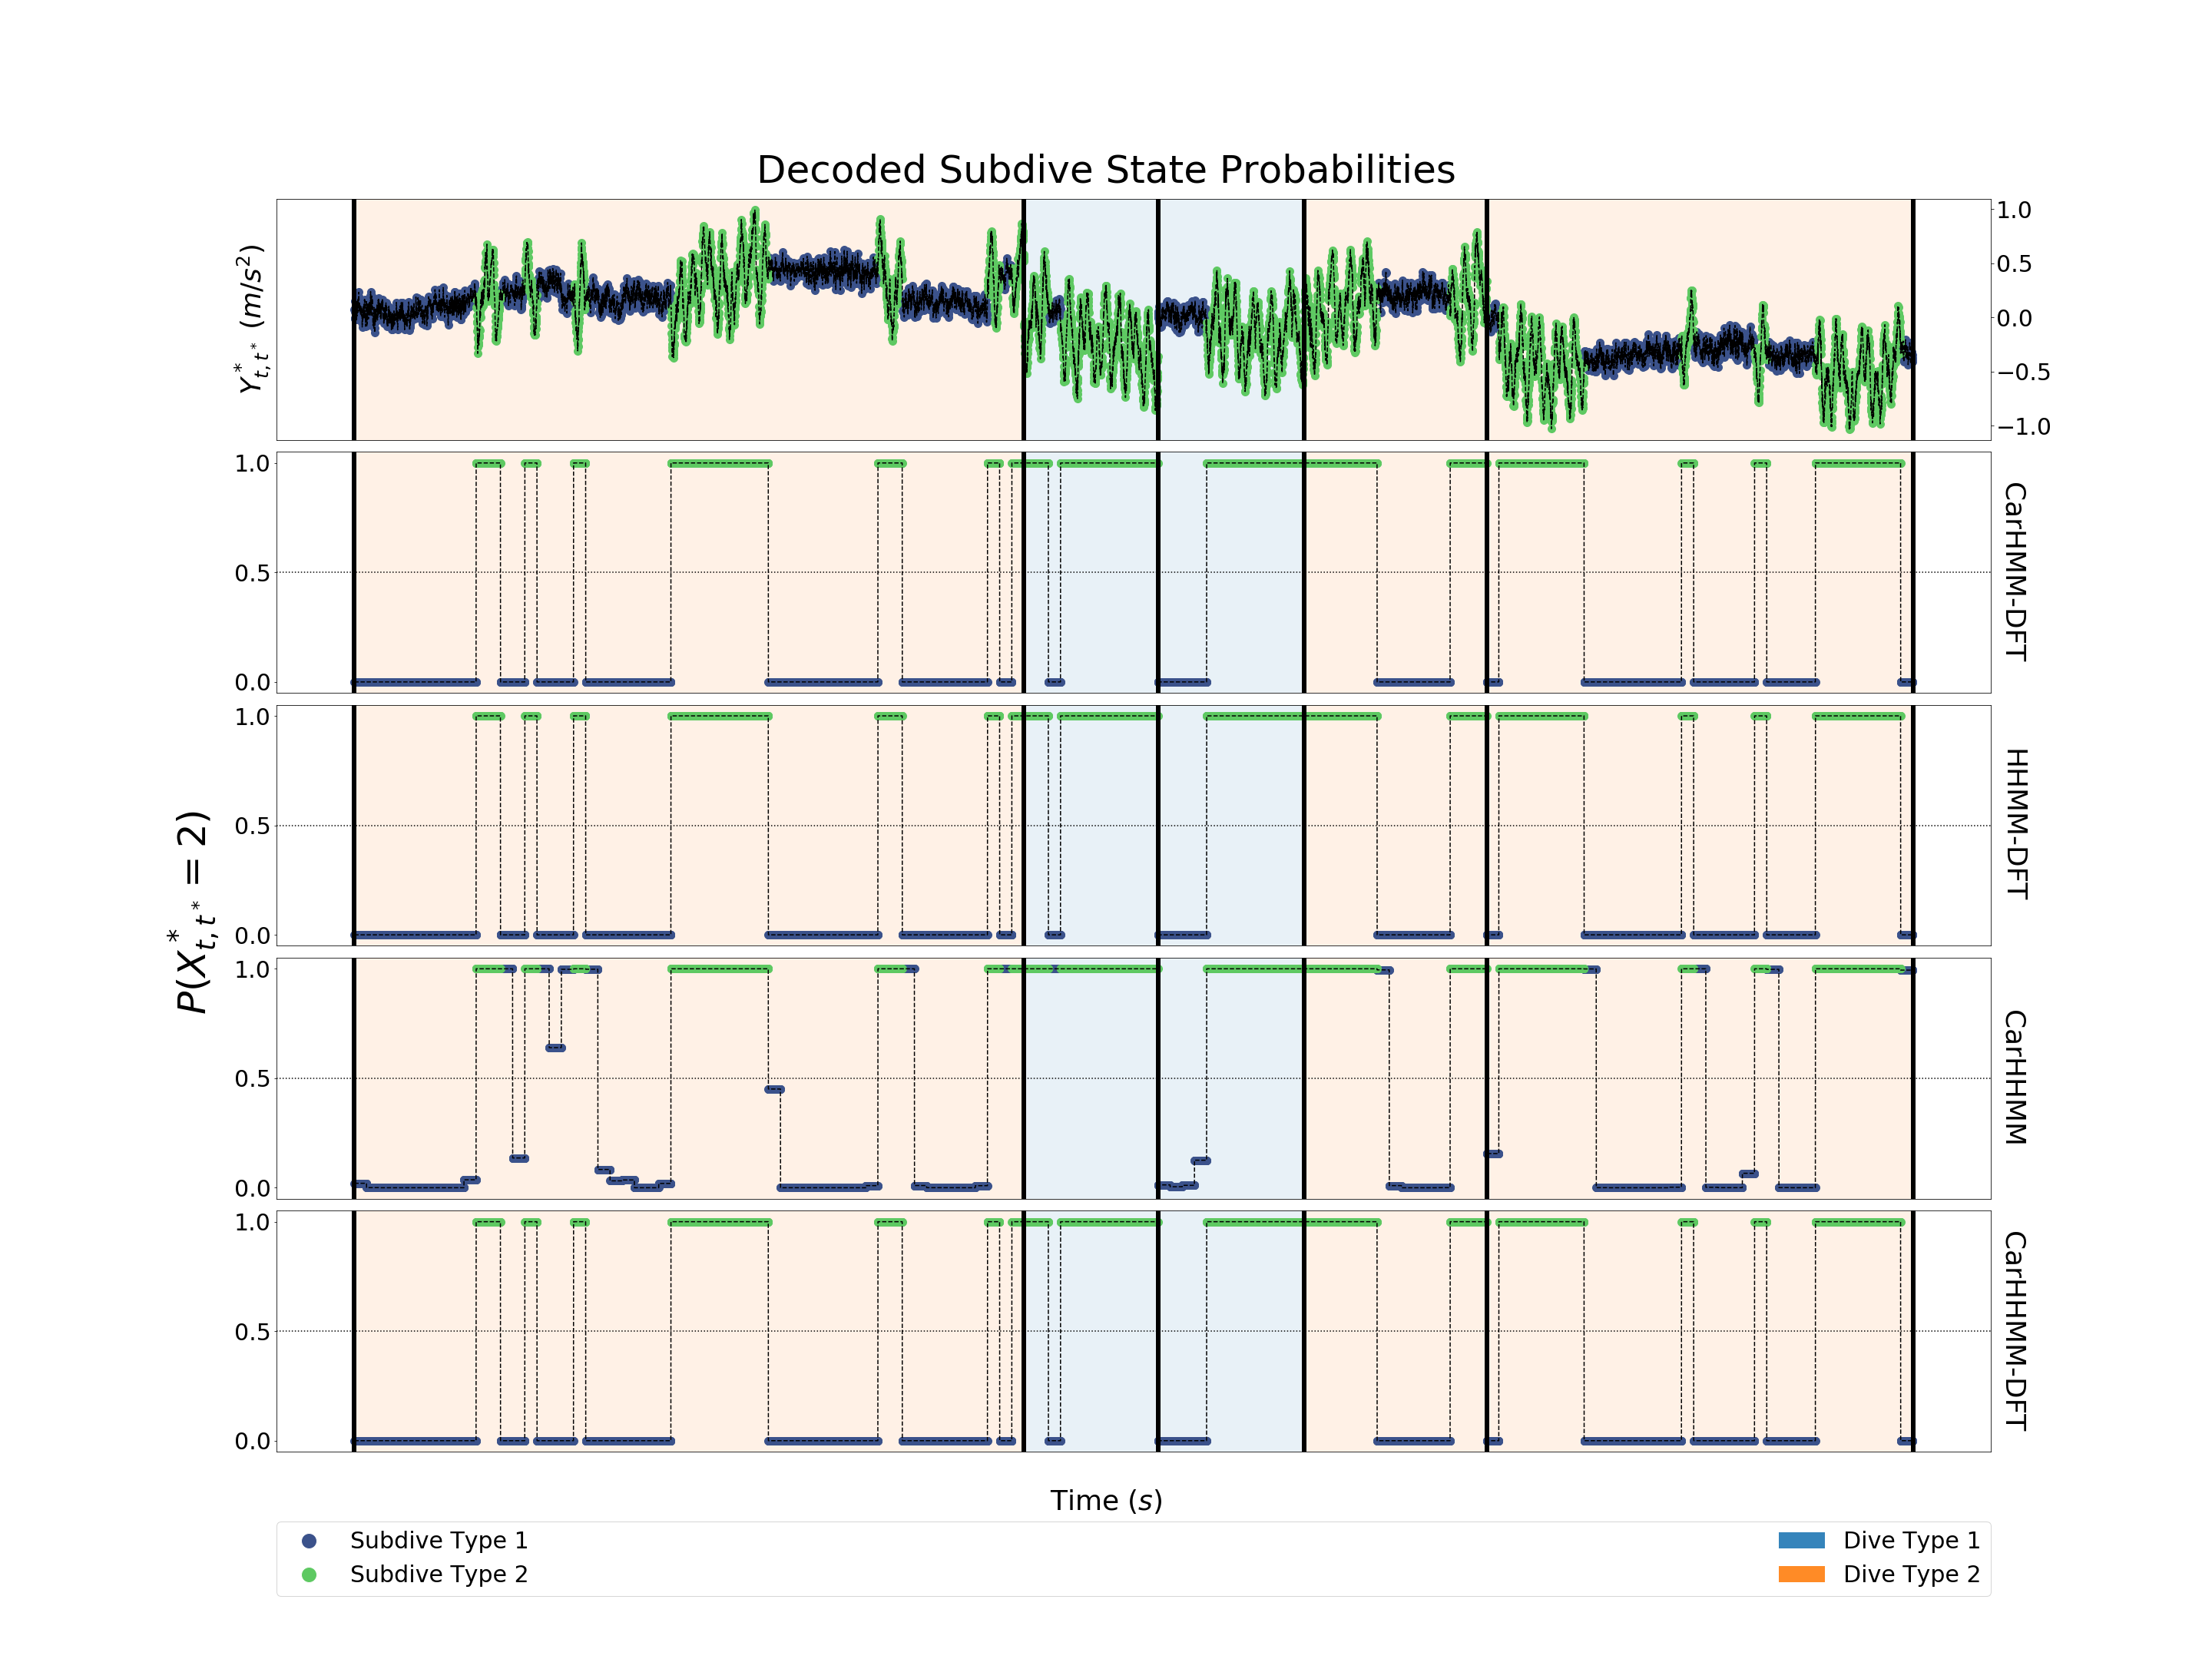
\includegraphics[width=5in]{Plots/Posterior_Fine_States.png}
        \caption{Fine-scale hidden process}
    \end{subfigure}
	\caption{Decoded state probabilities of each model. The color of the line corresponds to the true fine-scale state of the sub-dive process, while the color of the background corresponds to the true dive type of the simulated whale.}
	\label{fig:acc}
\end{figure}

%%% dive duration %%%
For the emission distributions of dive duration, estimates of standard error using the observed fisher information tended to be underestimates due to correlation between $\hat \mu$ and $\hat \sigma$. In addition, $\hat \sigma$ tends to underestimate $\sigma$ for all models, which is a finding consistent with properties of MLEs, especially because the sample size for a particular dive type is approximately 50 for each simulation. The CarHMM model in particular severely underestimates $\sigma$. This is likely due to the fact that dive duration follows a mixture of gammas rather than a gamma distribution, and the CarHMM does not have the machinery to capture this fact. A full table of parameter estimates for all models is shown in (table \ref{table:dive_duration}).


%%% Acceleration %%%
For acceleration ($Z^{*(1)}$), both the CarHMM-DFT and the CarHHMM-DFT regularly converged to the correct parameters with very little standard error. However, the fisher standard error regularly overestimated the standard error for $\hat \mu$ for both of these models. 
%This likely is due to the very large auto-correlation terms ($\phi^{(1)} = 0.99$ and $\phi^{(2)} = 0.95$) since as $\phi \to 1$, the value of $\mu$ does not matter in the likelihood evaluation as $\phi \to 1$ implies that $\mathbb{E}(Z^{*(1)}_{t,s^*}) = \phi*(Z^{*(1)}_{t,s^*-1}) + (1-\phi)\mu \to Z^{*(1)}_{t,s^*-1}$. 
The HHMM regularly overestimates the variance $Z^{*(1)}$ since it does not incorporate auto-correlation into the emission distribution of $Z^{*(1)}$, and the CarHHMM has large biases in many of its parameter estimates, especially in sub-dive state 2. 
%because it sees the ``wigliness" of the acceleration data as raw acceleration rather than as Fourier modes, which deflates the value of $\hat \phi$ and inflates the value of $\hat \sigma$. 
See (table \ref{table:acceleration}) for a detailed breakdown of parameter values for acceleration emission distributions.

%%% FoVeDBA %%%
The distribution of parameters for the Fourier sums ($Z^{*(2)}$) for all models except for the CarHHMM converge regularly to the correct values, and the observed fisher information standard errors are good approximation of the empirical standard error.
%The distribution of $Z^{*(2)}$ is very different between subdive states 1 and 2, so the signal is therefore very easy for each model to pick up on.
(Table \ref{table:FoVeDBA}) shows a detailed breakdown of the emission distribution of $Z^{*(2)}$ for all models.

%%% Gamma %%%

Estimates for $\Gamma$ for all models (except for the CarHMM-DFT) are very accurate, with empirical standard errors of approximately 0.02. This is significantly less than the observed fisher information estimate of standard error of approximately 0.08.
%likely because the distribution of $\hat \Gamma$ did not converge to a normal distribution in only 100 observed dives. 
For $\Gamma^*$, the HHMM-DFT and CarHHMM-DFT both showed practically no bias with standard errors on the order of $10^{-2}$. One notable exception is the standard error of $\hat \Gamma^{*(1)}_{12}$, whose standard error was on the order of $10^{-4}$, which is much lower than the observed Fischer information predicted. The CarHMM-DFT is mis-specified, so its results cannot be interpreted. The CarHHMM consistently underestimated the probability of a hidden state change on the sub-dive behavior. Again, one notable exception is $\hat \Gamma^{*(1)}_{12}$, which had almost no bias and was remarkably consistent. See (Table \ref{table:Gamma}) for a full list of estimates and standard errors.

\textcolor{red}{I also have plots corresponding to each table. For example, I have included figure \ref{fig:MLE_dist} as an example below for the emission distribution of the MLEs for dive duration of the CarHMM. Should I use those instead? But there are just SO many plots (4 models * 3 observations * 2 states = 24 plots)}

\begin{figure}[ht]
	\centering
	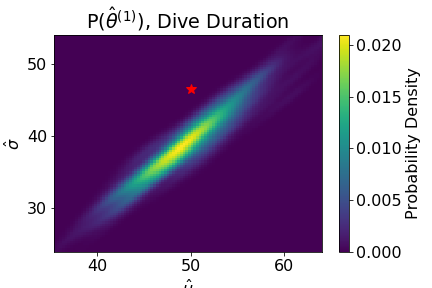
\includegraphics[width=5in]{../Plots/hmm_FV_MLE_density_dive_duration_-1.png}
	\caption{\textcolor{red}{KDE plot of $\hat \mu$ and $\hat \sigma$ for the dive duration emission distribution for the CarHMM. This plot is for Marie and Nancy to look over.}}
	\label{fig:MLE_dist}
\end{figure}

%%% Accuracy %%%

\begin{table}
\centering
\caption{Accuracies and run times for all models. All reported values are averages, and $\pm$ refers to the standard deviation.}
\scalebox{0.8}{
\begin{tabular}{ccccccc}
Model                      & \multicolumn{1}{c}{Training Time (Minutes)} & \multicolumn{1}{c}{Dive Type} & \multicolumn{1}{c}{Subdive Type} & \multicolumn{1}{c}{Dive Accuracy} & \multicolumn{1}{c}{Subdive Accuracy}  \\ \hline
\multirow{5}{*}{CarHMM}    & \multirow{5}{*}{$15.74 \pm 2.46$}   & Both                          & Both                             & -------------                     & $1.00 \pm 0.00$                       \\
                           &                                    & 1                             & 1                                & \multirow{2}{*}{-------------}    & $1.00 \pm 0.00$                       \\ 
                           &                                    & 1                             & 2                                &                                   & $1.00 \pm 0.00$                       \\ 
                           &                                    & 2                             & 1                                & \multirow{2}{*}{-------------}    & $1.00 \pm 0.00$                       \\ 
                           &                                    & 2                             & 2                                &                                   & $1.00 \pm 0.00$                       \\ \hline 
\multirow{5}{*}{HHMM}      & \multirow{5}{*}{$82.43 \pm 11.48$}   & Both                          & Both                             & $0.94 \pm 0.02$                   & $1.00 \pm 0.00$                       \\
                           &                                    & 1                             & 1                                & \multirow{2}{*}{$0.94\pm0.03$}    & $1.00 \pm 0.00$                       \\ 
                           &                                    & 1                             & 2                                &                                   & $1.00 \pm 0.00$                       \\ 
                           &                                    & 2                             & 1                                & \multirow{2}{*}{$0.94\pm0.03$}    & $1.00 \pm 0.00$                       \\ 
                           &                                    & 2                             & 2                                &                                   & $1.00 \pm 0.00$                       \\ \hline
\multirow{5}{*}{CarHHMM1}  & \multirow{5}{*}{$70.85 \pm 15.89$}   & Both                          & Both                             & $0.91 \pm 0.03$                   & $0.89 \pm 0.02$                       \\
                           &                                    & 1                             & 1                                & \multirow{2}{*}{$0.87\pm0.04$}    & $0.44 \pm 0.12$                       \\ 
                           &                                    & 1                             & 2                                &                                   & $1.00 \pm 0.00$                       \\ 
                           &                                    & 2                             & 1                                & \multirow{2}{*}{$0.95\pm0.03$}    & $0.81 \pm 0.04$                       \\ 
                           &                                    & 2                             & 2                                &                                   & $1.00 \pm 0.00$                       \\ \hline
\multirow{5}{*}{CarHHMM2}  & \multirow{5}{*}{$81.22 \pm 16.10$}   & Both                          & Both                             & $0.94 \pm 0.02$                   & $1.00 \pm 0.00$                       \\
                           &                                    & 1                             & 1                                & \multirow{2}{*}{$0.94\pm0.03$}    & $1.00 \pm 0.00$                       \\ 
                           &                                    & 1                             & 2                                &                                   & $1.00 \pm 0.00$                       \\ 
                           &                                    & 2                             & 1                                & \multirow{2}{*}{$0.94\pm0.03$}    & $1.00 \pm 0.00$                       \\ 
                           &                                    & 2                             & 2                                &                                   & $1.00 \pm 0.00$                       \\ \hline
\end{tabular}
}
\label{table:accuracy}
\end{table}

%%% dive duration %%%

\begin{table}
\centering
\caption{Estimates and standard errors of parameters for dive duration distribution for all four models. All reported values are averages, except for the Fisher observed standard error, which are medians. $\pm$ refers to the IQR.}
\scalebox{0.9}{
\begin{tabular}{ccccccc}
Model                      & \multicolumn{1}{c}{Parameter} & \multicolumn{1}{c}{Dive Type} & \multicolumn{1}{c}{Estimate} & \multicolumn{1}{c}{Bias} & \multicolumn{1}{c}{Empirical SE} & \multicolumn{1}{c}{Observed Fischer SE}           \\ \hline
\multirow{4}{*}{CarHMM}    & \multirow{2}{*}{$\mu$}        & 1                             & $49.72$                         & $-0.28$                     & $4.78$                             & $2.47 \pm 0.34$                             \\
                           &                               & ---                           & ---                            & ---                        & ---                                & ---                                         \\
                           & \multirow{2}{*}{$\sigma$}     & 1                             & $39.00$                         & $-7.51$                     & $5.05$                             & $2.50 \pm 0.40$                             \\
                           &                               & ---                           & ---                            & ---                        & ---                                & ---                                         \\ \hline
\multirow{4}{*}{HHMM}      & \multirow{2}{*}{$\mu$}        & 1                             & $19.99$                         & $-0.01$                     & $0.75$                             & $0.69 \pm 0.11$                             \\
                           &                               & 2                             & $79.85$                         & $-0.15$                     & $8.05$                             & $5.85 \pm 1.10$                             \\
                           & \multirow{2}{*}{$\sigma$}     & 1                             & $4.90$                         & $-0.10$                     & $0.61$                             & $0.53 \pm 0.10$                             \\
                           &                               & 2                             & $48.74$                         & $-1.26$                     & $6.50$                             & $5.15 \pm 1.02$                             \\ \hline
\multirow{4}{*}{CarHHMM 1} & \multirow{2}{*}{$\mu$}        & 1                             & $19.91$                         & $-0.09$                     & $0.77$                             & $0.71 \pm 0.12$                             \\
                           &                               & 2                             & $75.80$                         & $-4.20$                     & $7.72$                             & $5.32 \pm 0.98$                             \\
                           & \multirow{2}{*}{$\sigma$}     & 1                             & $4.73$                         & $-0.27$                     & $0.59$                             & $0.55 \pm 0.10$                             \\
                           &                               & 2                             & $49.48$                         & $-0.52$                     & $6.26$                             & $4.79 \pm 0.93$                             \\ \hline
\multirow{4}{*}{CarHHMM 2} & \multirow{2}{*}{$\mu$}        & 1                             & $19.99$                         & $-0.01$                     & $0.75$                             & $0.69 \pm 0.12$                             \\
                           &                               & 2                             & $79.85$                         & $-0.15$                     & $8.05$                             & $5.85 \pm 1.10$                             \\
                           & \multirow{2}{*}{$\sigma$}     & 1                             & $4.90$                         & $-0.10$                     & $0.61$                             & $0.53 \pm 0.10$                             \\
                           &                               & 2                             & $48.74$                         & $-1.26$                     & $6.50$                             & $5.15 \pm 1.02$                             
\end{tabular}
}
\label{table:dive_duration}
\end{table}


%%% Acceleration %%%

\begin{table}
\centering
\caption{Estimates and standard errors of parameters for $Z^{*(1)}_{t,t^*}$ for all four models. All reported values are averages, except for the Fisher observed standard error, which are medians. $\pm$ refers to the IQR.}
\scalebox{0.7}{
\begin{tabular}{ccccccc}
Model                      & \multicolumn{1}{c}{Parameter} & \multicolumn{1}{c}{Subdive Type} & \multicolumn{1}{c}{Estimate} & \multicolumn{1}{c}{Bias} & \multicolumn{1}{c}{Empirical SE} & \multicolumn{1}{c}{Observed Fischer SE}        \\ \hline
\multirow{6}{*}{CarHMM}    & \multirow{2}{*}{$\mu$}        & 1                             & $0.00$                         & $0.00$                     & $0.00$                             & $0.14 \pm 0.13$                             \\
                           &                               & 2                             & $0.00$                         & $0.00$                     & $0.01$                             & $0.06 \pm 0.02$                             \\
                           & \multirow{2}{*}{$\sigma$}     & 1                             & $0.05$                         & $-0.00$                     & $0.00$                             & $0.00 \pm 0.00$                             \\
                           &                               & 2                             & $0.10$                         & $-0.00$                     & $0.00$                             & $0.00 \pm 0.00$                             \\ 
                           & \multirow{2}{*}{$\phi$}       & 1                             & $0.99$                         & $-0.00$                     & $0.01$                             & $0.01 \pm 0.00$                             \\
                           &                               & 2                             & $0.95$                         & $-0.00$                     & $0.01$                             & $0.01 \pm 0.00$                             \\ \hline
\multirow{6}{*}{HHMM}      & \multirow{2}{*}{$\mu$}        & 1                             & $-0.01$                         & $-0.01$                     & $0.02$                             & $0.01 \pm 0.00$                             \\
                           &                               & 2                             & $-0.00$                         & $-0.00$                     & $0.02$                             & $0.01 \pm 0.00$                             \\
                           & \multirow{2}{*}{$\sigma$}     & 1                             & $0.25$                         & $0.20$                     & $0.04$                             & $0.00 \pm 0.00$                             \\
                           &                               & 2                             & $0.24$                         & $0.14$                     & $0.03$                             & $0.00 \pm 0.00$                             \\ 
                           & \multirow{2}{*}{$\phi$}       & 1                             & ------                         & ------                     & ------                             & ------                                      \\
                           &                               & 2                             & ------                         & ------                     & ------                             & ------                                      \\ \hline
\multirow{6}{*}{CarHHMM 1} & \multirow{2}{*}{$\mu$}        & 1                             & $0.00$                         & $0.00$                     & $0.00$                             & $0.08 \pm 0.04$                             \\
                           &                               & 2                             & $-0.01$                         & $-0.01$                     & $0.01$                             & $0.01 \pm 0.00$                             \\
                           & \multirow{2}{*}{$\sigma$}     & 1                             & $0.05$                         & $0.00$                     & $0.04$                             & $0.00 \pm 0.00$                             \\
                           &                               & 2                             & $0.27$                         & $0.17$                     & $0.01$                             & $0.00 \pm 0.00$                             \\ 
                           & \multirow{2}{*}{$\phi$}       & 1                             & $0.97$                         & $-0.02$                     & $0.10$                             & $0.00 \pm 0.00$                             \\
                           &                               & 2                             & $0.49$                         & $-0.46$                     & $0.05$                             & $0.02 \pm 0.00$                             \\ \hline
\multirow{6}{*}{CarHHMM 2} & \multirow{2}{*}{$\mu$}        & 1                             & $0.00$                         & $0.00$                     & $0.00$                             & $0.13 \pm 0.12$                             \\
                           &                               & 2                             & $0.00$                         & $0.00$                     & $0.00$                             & $0.06 \pm 0.02$                             \\
                           & \multirow{2}{*}{$\sigma$}     & 1                             & $0.05$                         & $-0.00$                     & $0.00$                             & $0.00 \pm 0.00$                             \\
                           &                               & 2                             & $0.10$                         & $-0.00$                     & $0.00$                             & $0.00 \pm 0.00$                             \\ 
                           & \multirow{2}{*}{$\phi$}       & 1                             & $0.99$                         & $-0.00$                     & $0.01$                             & $0.01 \pm 0.00$                             \\
                           &                               & 2                             & $0.95$                         & $-0.00$                     & $0.01$                             & $0.01 \pm 0.00$                             \\ \hline
\end{tabular}
}
\label{table:acceleration}
\end{table}


%%% FoVeDBA %%%

\begin{table}
\centering
\caption{Estimates and standard errors of parameters for $Z^{*(2)}_{t,t^*}$ for all four models. All reported values are averages, except for the Fisher observed standard error, which are medians. $\pm$ refers to the IQR.}
\scalebox{0.8}{
\begin{tabular}{ccccccc}
Model                      & \multicolumn{1}{c}{Parameter} & \multicolumn{1}{c}{Subdive Type} & \multicolumn{1}{c}{Estimate} & \multicolumn{1}{c}{Bias} & \multicolumn{1}{c}{Empirical SE} & \multicolumn{1}{c}{Observed Fischer SE}        \\ \hline
\multirow{4}{*}{CarHMM}    & \multirow{2}{*}{$\mu$}        & 1                             & $10.10$                         & $-0.00$                     & $0.09$                             & $0.08 \pm 0.01$                             \\
                           &                               & 2                             & $305.97$                         & $0.03$                     & $0.54$                             & $0.51 \pm 0.03$                             \\
                           & \multirow{2}{*}{$\sigma$}     & 1                             & $3.18$                         & $-0.00$                     & $0.07$                             & $0.06 \pm 0.01$                             \\
                           &                               & 2                             & $17.46$                         & $-0.03$                     & $0.37$                             & $0.36 \pm 0.02$                             \\ \hline
\multirow{4}{*}{HHMM}      & \multirow{2}{*}{$\mu$}        & 1                             & $10.10$                         & $-0.00$                     & $0.09$                             & $0.08 \pm 0.01$                             \\
                           &                               & 2                             & $305.97$                         & $0.03$                     & $0.54$                             & $0.51 \pm 0.03$                             \\
                           & \multirow{2}{*}{$\sigma$}     & 1                             & $3.18$                         & $-0.00$                     & $0.07$                             & $0.06 \pm 0.01$                             \\
                           &                               & 2                             & $17.46$                         & $-0.03$                     & $0.37$                             & $0.36 \pm 0.02$                             \\ \hline
\multirow{4}{*}{CarHHMM 1} & \multirow{2}{*}{$\mu$}        & 1                             & ------                         & ------                     & ------                             & ------                                      \\
                           &                               & 2                             & ------                         & ------                     & ------                             & ------                                      \\
                           & \multirow{2}{*}{$\sigma$}     & 1                             & ------                         & ------                     & ------                             & ------                                      \\
                           &                               & 2                             & ------                         & ------                     & ------                             & ------                                      \\ \hline
\multirow{4}{*}{CarHHMM 2} & \multirow{2}{*}{$\mu$}        & 1                             & $10.10$                         & $-0.00$                     & $0.09$                             & $0.08 \pm 0.01$                             \\
                           &                               & 2                             & $305.97$                         & $0.03$                     & $0.54$                             & $0.51 \pm 0.03$                             \\
                           & \multirow{2}{*}{$\sigma$}     & 1                             & $3.18$                         & $-0.00$                     & $0.07$                             & $0.06 \pm 0.01$                             \\
                           &                               & 2                             & $17.46$                         & $-0.03$                     & $0.37$                             & $0.36 \pm 0.02$                             
\end{tabular}
}
\label{table:FoVeDBA}
\end{table}

% Gamma
\begin{table}[t]
\centering
\caption{Estimates and standard errors of $\Gamma$ and $\Gamma^*$ for all four models. All reported values are averages except for the observed fisher SE, which is a median. $\pm$ refers to the IQR.}
\scalebox{0.7}{
\begin{tabular}{ccccccc}
Model                        & \multicolumn{1}{c}{Parameter} & \multicolumn{1}{c}{Estimate}   & \multicolumn{1}{c}{Bias} & \multicolumn{1}{c}{Empirical SE} & \multicolumn{1}{c}{Observed Fischer SE}     \\ \hline
\multirow{6}{*}{HHMM-DFT}    & $\Gamma_{12}$                 & $0.50$                         & $-0.00$                   & $0.03$                           & $0.08 \pm 0.01$                             \\
                             & $\Gamma_{21}$                 & $0.50$                         & $-0.00$                   & $0.03$                           & $0.08 \pm 0.01$                             \\
                             & $\Gamma^{*(1)}_{12}$          & $0.50$                         & $0.00$                   & $0.00$                           & $0.07 \pm 0.01$                             \\
                             & $\Gamma^{*(1)}_{21}$          & $0.10$                         & $0.00$                   & $0.02$                           & $0.02 \pm 0.00$                             \\
                             & $\Gamma^{*(2)}_{12}$          & $0.20$                         & $-0.00$                   & $0.01$                           & $0.01 \pm 0.00$                             \\
                             & $\Gamma^{*(2)}_{21}$          & $0.30$                         & $-0.00$                   & $0.02$                           & $0.02 \pm 0.00$                             \\ \hline
\multirow{6}{*}{CarHMM-DFT}  & $\Gamma_{12}$                 & ------                         & ------                   & ------                           & ------                                      \\
                             & $\Gamma_{21}$                 & ------                         & ------                   & ------                           & ------                                      \\
                             & $\Gamma^{*(1)}_{12}$          & $0.23$                         & ------                   & $0.01$                           & $0.00 \pm 0.00$                             \\
                             & $\Gamma^{*(1)}_{21}$          & $0.23$                         & ------                   & $0.02$                           & $0.00 \pm 0.00$                             \\
                             & $\Gamma^{*(2)}_{12}$          & ------                         & ------                   & ------                           & ------                                      \\
                             & $\Gamma^{*(2)}_{21}$          & ------                         & ------                   & ------                           & ------                                      \\ \hline
\multirow{6}{*}{CarHHMM}     & $\Gamma_{12}$                 & $0.49$                         & $-0.01$                   & $0.02$                           & $0.08 \pm 0.01$                             \\
                             & $\Gamma_{21}$                 & $0.50$                         & $0.00$                   & $0.02$                           & $0.08 \pm 0.01$                             \\
                             & $\Gamma^{*(1)}_{12}$          & $0.50$                         & $-0.00$                   & $0.00$                           & $0.23 \pm 0.19$                             \\
                             & $\Gamma^{*(1)}_{21}$          & $0.04$                         & $-0.06$                   & $0.02$                           & $0.01 \pm 0.00$                             \\
                             & $\Gamma^{*(2)}_{12}$          & $0.11$                         & $-0.09$                   & $0.02$                           & $0.01 \pm 0.00$                             \\
                             & $\Gamma^{*(2)}_{21}$          & $0.11$                         & $-0.19$                   & $0.03$                           & $0.01 \pm 0.00$                             \\ \hline
\multirow{6}{*}{CarHHMM-DFT} & $\Gamma_{12}$                 & $0.50$                         & $-0.00$                   & $0.03$                           & $0.08 \pm 0.01$                             \\
                             & $\Gamma_{21}$                 & $0.50$                         & $-0.00$                   & $0.03$                           & $0.08 \pm 0.01$                             \\
                             & $\Gamma^{*(1)}_{12}$          & $0.50$                         & $0.00$                   & $0.00$                           & $0.07 \pm 0.01$                             \\
                             & $\Gamma^{*(1)}_{21}$          & $0.10$                         & $0.00$                   & $0.02$                           & $0.02 \pm 0.00$                             \\
                             & $\Gamma^{*(2)}_{12}$          & $0.20$                         & $-0.00$                   & $0.01$                           & $0.01 \pm 0.00$                             \\
                             & $\Gamma^{*(2)}_{21}$          & $0.30$                         & $-0.00$                   & $0.02$                           & $0.02 \pm 0.00$                             \\ \hline

\end{tabular}
}
\label{table:Gamma}
\end{table}